%% Public domain image from
%% http://www.public-domain-image.com/objects/computer-chips/slides/six-computers-chips-circuits.html
\renewcommand\chapterillustration{Math_matrix/chapterImage}



\chapter{행렬}
\index{행렬}\index{matrix}

행렬은 1차 방정식의 풀이에 아주 오래 전부터 사용되어 왔다. 하지만 행렬은 그 특성이 정확히 파악되지 않고 1800년대까지는 배열(array)이라는 이름으로 알려져 있었다.
기원전 10세기에서 기원전 2세기 사이에 여러 세대에 걸쳐 쓰여진 중국의 구장산술(九章算術)에 연립 방정식을 풀기 위해 배열을 적용하는 예가 처음으로 소개되었다.
여기에 판별식의 개념도 등장한다. 1545년에야 이탈리아 수학자 지롤라모 카르다노(Girolamo Cardano)가 그의 저서 "위대한 기술(Ars Magna)"를 통해 이 기법을 유럽에 전했다\cite{wiki:matrix}.

이후 오랜 기간 동안 많은 수학자들이 이 행렬을 다루며 다양한 성질을 발견하게 된다. 이 장에서는 게임이나 실시간 그래픽스 콘텐츠를 구현하는 데에 필요한
기본적인 행렬 개념을 이해할 것이다. 행렬은 공간을 나루는 데에 필요한 유용한 도구이다.
공간 내의 점들을 이떤 위치에서 다른 위치로 옮겨 놓는 다양한 변환이 행렬을 이용하여 표현될 수 있으며, 
특정 좌표계를 다른 좌표계로 변경하는 작업과 같이 공간을 모델링하는 다양한 문제에서 효율적이며 효과적인 계산 도구를 제공한다.

\section{행렬이란 무엇인가?}
\index{행벡터}\index{열벡턱}
\index{row vector}\index{column vector}

행렬은 2차원으로 배열된 수라고 할 수 있다. 가로와 세로로 줄지어 있는 수들이다.
가로 줄을 행(row)이라 하고, 세로 줄을 열(column)이라고 한다.

예를 들어 $m$ 개의 행과 $n$ 개의 열로 이루어진 행렬은 $\mathbf A$는 다음과 같은 모양이다.

$$\mathbf A = \left [ 
\begin{array}{cccccc}
a_{11} & a_{12} & \cdots & a_{1j} & \cdots & a_{1n} \\
a_{21} & a_{22} & \cdots & a_{2j} & \cdots & a_{2n} \\
\vdots & \vdots & \ddots &   \vdots   & \ddots & \vdots \\
a_{i1} & a_{i2} & \cdots & a_{ij} & \cdots & a_{in} \\
\vdots & \vdots & \ddots & \vdots & \ddots & \vdots\\
a_{m1} & a_{m2} & \cdots & a_{mj} & \cdots & a_{mn} \\
\end{array}
\right ]$$

이 행렬은 $m \times n$ 행렬이며, $\mathbf A \in \mathbb R^{m\times n}$로 표현한다.
이 경우 각 행은 $n$ 개의 원소를 가진 벡터라고 생각할 수 있다. 이 벡터를 행벡터(row vector)라고 부르며,
하나의 $\mathbf A$에는 총 $m$ 개의 행벡터가 있다. 
또한 이 행렬의 각 열은 $m$ 개의 원소를 가진 벡터라고 할 수 있으며, 이를 열벡터(column vector)라고 부른다.
이 행렬에는 총 $n$ 개의 열벡터가 존재한다. 

$\mathbf A$를 행벡터 $\mathbf v_i^r$로 표현하면 다음과 같다.
$$\mathbf A = \left [ 
\begin{array}{c}
\mathbf v_1^r\\
\mathbf v_2^r\\
\vdots\\
\mathbf v_m^r
\end{array}
\right ]$$

$\mathbf A$를 열벡터 $\mathbf v_j^c$로 표현하면 다음과 같다.
$$\mathbf A = \left [ 
\begin{array}{cccc}
\mathbf v_1^c & \mathbf v_2^c & \cdots & \mathbf v_n^c
\end{array}
\right ]$$

이렇게 행렬을 벡터의 모음으로 이해하는 방식을 그림 \ref{fig:matrix:matrixAsVectorCollection}와 같이 표현할 수 있다.
\begin{figure}[h!]
  \centering
    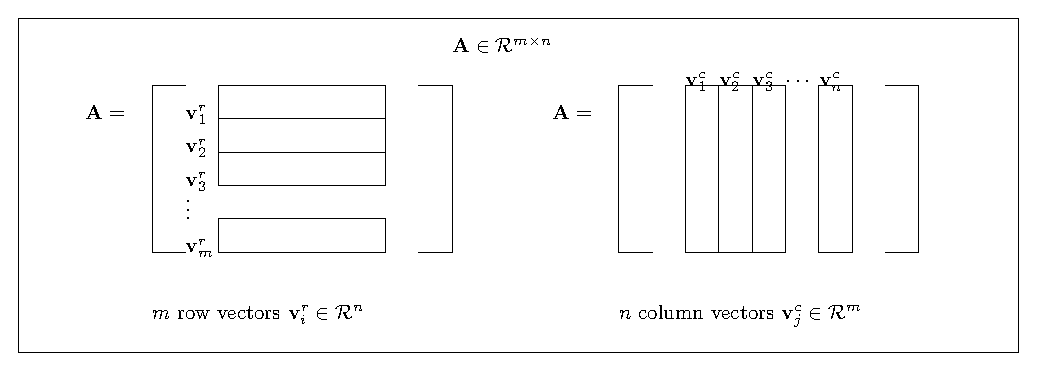
\includegraphics[width=12cm]{Math_matrix/matrixAsVectorCollection.eps}
    \caption{$\mathbf A \in \mathbb R^{m \times n}$을 벡터의 모음으로 이해하는 방법}
    \label{fig:matrix:matrixAsVectorCollection}
\end{figure}

\section{행렬의 기본적 이해}

이 절에서는 행렬에 대한 기본적인 이해를 할 것이다.

\subsection{정방행렬(square matrix)}
\index{정방행렬}\index{행렬!정방행렬}\index{정사각행렬}\index{행렬!정사각행렬}
\index{square matrix}\index{matrix!square}

정방행렬, 혹은 정사각형 행렬은 행과 열의 수가 동일한 행렬이다. 다시 말해 $\mathbf A \in \mathbb R^{n \times n}$인 행렬이다.
정방행렬은 물리 문제에서 운동을 다루거나 그래픽스에서 변환을 다룰 때에 빈번히 나타난다.
다음 행렬 $\mathbf A$는 $3\times 3$의 정사각 행렬이다.

\begin{eqnarray}
\mathbf A = \left [ 
\begin{array}{ccc}
a_{11} & a_{12} & a_{13} \\
a_{21} & a_{22} & a_{23} \\
a_{31} & a_{32} & a_{33} \\
\end{array}
\right ]
\label{eq:matrix33example}
\end{eqnarray}


\subsection{전치행렬(transpose matrix)}
\index{전치행렬}\index{행렬!전치}
\index{transpose matrix}\index{matrix!transpose}

어떤 행렬 $\mathbf A$의 전치행렬은 $\mathbf A^{\rm T}$로 쓴다.
만약 $\mathbf B = \mathbf A^{\rm T}$라면 행렬 $\mathbf A$와 $\mathbf B$의 원소들 사이에는 다음과 같은
관계가 성립한다.

$$
\mathbf B = \mathbf A^{\rm T} \Rightarrow b_{ij} = a_{ji}
$$

따라서, $m \times n$ 행렬의 전치는 $n \times m$ 행렬이 된다.

$$
\mathbf A \in \mathbb R^{m \times n} \Rightarrow \mathbf B \in \mathbb R^{n \times m}
$$

전치행렬은 또한 다음과 같은 성질을 갖는다.

$$
\mathbf (\mathbf A^{\rm T})^{\rm T} = A
$$
$$
(\mathbf A + \mathbf B)^{\rm T} = \mathbf A^{\rm T} + \mathbf B^{\rm T}
$$
$$
(k\mathbf A)^{\rm T} = k \mathbf A^{\rm T}
$$
$$
(\mathbf {AB})^{\rm T} = \mathbf B^{\rm T} \mathbf A^{\rm T}
$$

전치행렬은 다양하게 사용될 수 있는데, 그래픽스(graphics) 분야에서 매우 유용한 사용 방법은 회전 변환 행렬의 역행렬을 구할 때이다.
3차원 공간의 회전 변환은 $3 \times 3$ 행렬로 표현할 수 있는데, 이 행렬은 정규직교(orthonormal)한 특성을 갖는다.
그리고 정규직교 행렬의 역행렬은 그 행렬의 전치임이 알려져 있다. 따라서 회전변환의 역변환은 전치행렬이 된다.
이 부분은 변환에 관한 장에서 다시 다루어질 것이다.

\subsection{대각행렬(diagonal matrix)}
\index{대각행렬}\index{행렬!대각행렬}
\index{diagonal matrix}\index{matrix!diagonal}

대각행렬을 이해하기 위해서는 대각 성분부터 이해하자.
대각성분은 어떤 행렬 $\mathbf A$의 $i$ 행 $j$ 열 성분을 $a_{ij}$라고 표현할 때, $i=j$인 성분이다.
식 \ref{eq:matrix33example}의 행렬이 가진 대각성분은 $a_{11}, a_{22}, a_{33}$ 세 개이다.

대각행렬은 대각성분을 제외한 다른 모든 성분의 값이 0인 행렬이다. 따라서 다음과 같은 행렬이 대각행렬이다.

$$\mathbf A = \left [ 
\begin{array}{ccc}
a_{11} & 0 & 0 \\
0 & a_{22} & 0 \\
0 & 0 & a_{33} \\
\end{array}
\right ]$$

대각행렬을 다른 행렬과 곱했을 때에는 어떤 성질을 가지는지 살펴 보자.
어떤 $3 \times 3$ 대각행렬을 $\mathbf D$라 부르고,
1,2,3 행 대각성분을 각각 $d_1, d_2, d_3$라고 하자.
다른 어떤 $3 \times 3$ 행렬이 식 \ref{eq:matrix33example}의  $\mathbf A$라고 하자.
대각행렬 $\mathbf D$와 행렬 $\mathbf A$의 곱은 다음과 같다.
$$
\mathbf{DA} = \left [
\begin{array}{ccc}
d_1 a_{11} & d_1 a_{12} & d_1 a_{13} \\
d_2 a_{21} & d_2 b_{22} & d_2 b_{23} \\
d_3 a_{31} & d_3 b_{32} & d_3 b_{33}
\end{array}
\right ]
,~~~~
\mathbf{AD} = \left [
\begin{array}{ccc}
d_1 a_{11} & d_2 a_{12} & d_3 a_{13} \\
d_1 a_{21} & d_2 b_{22} & d_3 b_{23} \\
d_1 a_{31} & d_2 b_{32} & d_3 b_{33}
\end{array}
\right ]
$$

어떤 열벡터 $\mathbf v \in \mathbb R^3$이 $(v_1, v_2, v_3)^{\rm T}$라고 하자. 대각행렬 $\mathbf D$와 벡터 $\mathbf v$의 곱은 다음과 같다.
$$
\mathbf {Dv} = 
\left [ 
\begin{array}{ccc}
a_{11} & 0 & 0 \\
0 & a_{22} & 0 \\
0 & 0 & a_{33} \\
\end{array}
\right ]
\left [
\begin{array}{c}
v_1 \\
v_2 \\
v_3 \\
\end{array}
\right ]
=
\left [
\begin{array}{c}
d_1 v_1 \\
d_2 v_2 \\
d_3 v_3 \\
\end{array}
\right ]
$$


비슷하게 행벡터 $\mathbf v^{\rm T}$와 대각행렬의 곱은 다음과 같다.

$$
\mathbf v^{\rm T} \mathbf D = 
\left [
\begin{array}{ccc}
v_1 & v_2 & v_3 \\
\end{array}
\right ]
\left [ 
\begin{array}{ccc}
a_{11} & 0 & 0 \\
0 & a_{22} & 0 \\
0 & 0 & a_{33} \\
\end{array}
\right ]
=
\left [
\begin{array}{ccc}
d_1 v_1 & d_2 v_2 &d_3 v_3 \\
\end{array}
\right ]
$$

\section{행렬의 연산}

\subsection{행렬의 덧셈과 뺄셈}
\index{행렬!덧셈과 뺄셈}
\index{matrix!addition and subtraction}

두 행렬의 덧셈은 동일한 크기의 행렬 사이에 정의된다.
따라서 $\mathbb R^{m \times n}$에 속한 행렬은 이와 동일한  $\mathbb R^{m \times n}$의 행렬과만 덧셈이 정의되며,
얻어지는 결과 역시  $\mathbb R^{m \times n}$에 속한 행렬이다.
뺄셈 역시 동일한 차원의 행렬들 사이에 정의된다.

$$\mathbf A \in \mathbb R^{m \times n}  \wedge \mathbf A + \mathbf B = \mathbf C \Rightarrow \mathbf B, \mathbf C \in \mathbb R^{m \times n}$$
$$\mathbf A \in \mathbb R^{m \times n}  \wedge \mathbf A - \mathbf B = \mathbf D \Rightarrow \mathbf B, \mathbf D \in \mathbb R^{m \times n}$$

행렬과 덧셈과 뺄셈은 동일한 행과 열에 있는 성분을 서로 더하고, 빼서 원래의 자리에 기록하면 된다.

$$\mathbf A + \mathbf B = \mathbf C \Rightarrow c_{ij} = a_{ij} + b_{ij}$$
$$\mathbf A - \mathbf B = \mathbf D \Rightarrow d_{ij} = a_{ij} - b_{ij}$$


\subsection{행렬의 곱셈}
\index{행렬!곱셈}
\index{matrix!multiplication}

어떤 행렬 $\mathbf A$가 $\mathbb R^{m \times n}$의 원소라고 하자. 이 행렬의 뒤에 곱해질 수 있는 행렬 $\mathbf B$가 있다면,
이것은 반드시 $\mathbb R^{n \times x}$의 원소이다. 그리고 이 둘의 곱은  $\mathbf {AB} = \mathbf C \in \mathbb R^{m \times x}$이다.

$\mathbf A$의 앞에 $\mathbf B$를 곱한다면 $\mathbf B \in \mathbb R^{x \times m}$이어야 하며, 
그 결과는 $\mathbf {BA} = \mathbf D \in \mathbb R^{x \times n}$이다.

다음과 같은 곱셈을 살펴 보자.
$$\mathbf A \in \mathbb R^{m \times n}$$
$$\mathbf B \in \mathbb R^{n \times x}$$
$$\mathbf {AB} = \mathbf C \in \mathbb R^{m \times x}$$


이때, $\mathbf C$의 $i$ 행 $j$ 열 원소 $c_{ij}$의 값은 다음과 같이 구해진다.

\begin{eqnarray}
c_{ij} & =  &a_{i1}b_{1j} + a_{i2}b_{2_j} + \cdots + a_{in}b_{nj} \\ \nonumber
    & = & \sum_{k=1}^n a_{ik} b_{kj}
\end{eqnarray}

행렬 $\mathbf A$의 $i$ 번째 행 벡터를 $\mathbf A_{i,*}$라고 하고, $j$ 번째 열 벡터를 $\mathbf B_{*,j}$라고 하면,
위의 식은 다음과 같이 다시 쓸 수 있다.

\begin{eqnarray}
c_{ij} & =  & \mathbf A_{i,*}^{\rm T} \cdot \mathbf B_{*,j}
\end{eqnarray}

\subsection{행렬과 스칼라의 곱}
\index{matrix!scalar multiplication}\index{행렬!스칼라 곱}

행렬에 스칼라를 곱하는 연산은 해당 스칼라 값을 행렬의 모든 원소에 곱하면 된다.

$$k \mathbf A  = \mathbf B \Rightarrow b_{ij} = k a_{ij}$$

\subsection{행렬의 연산 법칙}
\index{행렬!연산 법칙}

행렬은 다음과 같은 연산 법칙을 가진다.

\subsubsection{덧셈}

$$\mathbf A + \mathbf B = \mathbf B + \mathbf A$$
$$(\mathbf A + \mathbf B ) + \mathbf C = \mathbf A + ( \mathbf B + \mathbf C ) $$
$$ \mathbf A + 0 = 0 + \mathbf A = \mathbf A$$
$$ \mathbf A + (- \mathbf A ) = 0$$

이때, 0은 $\mathbf A$와 같은 차원의 행렬로 모든 원소가 0인 행렬이다.

\subsubsection{스칼라 곱셈}

$$(k+l) \mathbf A = k \mathbf A + l \mathbf A$$
$$k (\mathbf A + \mathbf B ) = k \mathbf A + k \mathbf B$$
$$(kl) \mathbf A = k (l \mathbf A)$$
$$ (-1) \mathbf A = -\mathbf A$$
$$ 0 \mathbf A = 0$$

\subsection{행렬 곱셈}

$$\mathbf{AB} \neq \mathbf {BA}$$
$$\mathbf{A(BC)} = \mathbf{(AB)C}$$
$$\mathbf{A(B+C)} = \mathbf {AB} + \mathbf {AC}$$
$$\mathbf{(A+B)C} = \mathbf{AC} + \mathbf{BC}$$
$$\mathbf{AI} = \mathbf{IA} = \mathbf A$$
$$k \mathbf{AB} = (k\mathbf A)\mathbf B = \mathbf A k \mathbf B$$

이때, $\mathbf I$는 항등행렬 혹은 단위행렬이라 부르며, 대각성분이 모두 1이며, 비대각성분은 모두 0인 행렬이다.

\section{행렬식}
\index{matrix!determinant}\index{행렬!행렬식}\index{행렬식}

행렬식은 정방행렬에서 정의된다. 어떤 행렬 $\mathbf A$의 행렬식은 $det \mathbf A$, $det(\mathbf A)$, 또는 $|\mathbf A|$로 표현한다.
행렬식을 계산하기 위해서는 다음과 같은 개념에 대한 이해를 해야 한다.
\begin{itemize}
\item 소행렬식(minor)
\item 여인자(cofactor)
\end{itemize}

\subsection{소행렬식}
\index{matrix!minor}\index{행렬!소행렬식}\index{소행렬식}

행렬 $\mathbf A$가 $\mathbb R^{m \times n}$에 속한 행렬이라고 할 때, 이 행렬은
모두 $m \times n$개의 소행렬식(minor) $M_{ij}$를 가진다.
이때 각 $M_{ij}$는 $\mathbf A$ 행렬의 $i$ 행 벡터 전체와 $j$ 열 벡터 전체를 제거하고 얻어지는 행렬($\in \mathbb R^{m-1 \times n-1}$)의 
행렬식이다.

\subsection{여인자}
\index{matrix!cofactor}\index{행렬!여인자}\index{여인자}

행렬 $\mathbf A$의 여인자는 소행렬식이 구해지는 위치마다 결정된다.
따라서 $m \times n$개의 여인자 $C_{ij}$가 존재하며, 다음과 같이 정의된다.

$$C_{ij} = (-1)^{i+j} M_{ij}$$

행렬 $\mathbf A \in \mathbb R^{m \times n}$의 $i$ 행, $j$ 열에서 정의되는 여인자를 $C_{ij}$라고 하고, 행렬의 각 성분은 $A_{ij}$라고 하면,
이 행렬의 행렬식은 다음과 같다.

\begin{eqnarray}
det \mathbf A &= | \mathbf A | &= \sum_{j=1}^n A_{1j} C_{1j} = \sum_{j=1}^n A_{2j} C_{2j} = \cdots = \sum_{j=1}^n A_{mj} C_{mj} \\ \nonumber
& &= \sum_{i=1}^m A_{i1} C_{i1} = \sum_{i=1}^m A_{i2} C_{i2} = \cdots = \sum_{j=1}^n A_{in} C_{in} 
\end{eqnarray}

이것은 행렬 $\mathbf A$에서 임의의 행 벡터 $\mathbf A_{i,*}$를 선택하고, 여인자 $C_{ij}$를 원소로 하는 행렬 $\mathbf C$의 동일한 위치에 있는 행 벡터 $\mathbf C_{i,*}$를 선택하여 둘의 내적 $\mathbf A_{i,*} \mathbf C_{i,*}^{\rm T}$를 구하는 것이다.
또한, 이 값은 $\mathbf A$에서 임의의 열 벡터 $\mathbf A_{*,j}$를 선택하고, 행렬 $\mathbf C$의 동일한 위치에 있는 열 벡터 $\mathbf C_{*,j}$를 선택하여 둘의 내적 $\mathbf A_{*,j}^{\rm T} \mathbf C_{*,j}$를 구하는 것이다.

\begin{eqnarray}
det \mathbf A = | \mathbf A | = \mathbf A_{i,*} \mathbf C_{i,*}^{\rm T} = \mathbf A_{*,j}^{\rm T} \mathbf C_{*,j}
\end{eqnarray}

%%%%%%%%% 예제 시작
\hrule

\noindent \colorbox{lightgray}{\begin{minipage}{6cm}예제\end{minipage}} 


\noindent  어떤 행렬 $\mathbf A$가 있다. 이 행렬의 원소는 다음과 같다. 이 행렬의 행렬식을 구하라.
$$
\left [
\begin{array}{cc}
A_{11} & A_{12} \\
A_{21} & A_{22}
\end{array}
\right ]
$$

\noindent \colorbox{lightgray}{\begin{minipage}{6cm}정답\end{minipage}} 

우선 여인자를 구한다. 여인자 $M_{ij}$를 $i$ 행 $j$ 열 원소로 하는 행렬을 $\mathbf M$이라고 하자. 그러면 이 행렬은 다음과 같다.
$$
\mathbf M = 
\left [
\begin{array}{cc}
M_{11} & M_{12} \\
M_{21} & M_{22}
\end{array}
\right ] = 
\left [
\begin{array}{cc}
det \left [ A_{22} \right ] &
det \left [ A_{21} \right ] \\
det \left [ A_{12} \right ] &
det \left [ A_{11} \right ] 
\end{array}
\right ]
$$
원소가 하나인 행렬의 행렬식은 그 원소의 값이므로, $\mathbf M$은 다음과 같다.
$$
\mathbf M = 
\left [
\begin{array}{cc}
A_{22} & A_{21} \\
A_{12} & A_{11} 
\end{array}
\right ]
$$

여인자의 정의에 따라, 여인자로 구성된 행렬 $\mathbf C$는 다음과 같다.
$$
\mathbf C = 
\left [
\begin{array}{cc}
(-1)^{1+1} A_{22} & (-1)^{1+2} A_{21} \\
(-1)^{2+1} A_{12} & (-1)^{2+2} A_{11} 
\end{array}
\right ]
= \left [
\begin{array}{cc}
A_{22} & -A_{21} \\
-A_{12} & A_{11} 
\end{array}
\right ]
$$

$\mathbf A$의 임의의 행 벡터를 선택할 수 있으므로 우선 1행을 가지고 오자. 그리고 여인자 행렬 $\mathbf C$의 1행을 가지고 와서, 두 행 벡터의 내적을 
구하면 다음과 같다.
\begin{eqnarray}
det \mathbf A & = \mathbf A_{1,*}  \mathbf C_{1,*}^{\rm T} & =  A_{11}  A_{22} +  A_{12} (-  A_{21}) \\ \nonumber
& & =   A_{11}  A_{22} -  A_{12}  A_{21} \\ \nonumber
\end{eqnarray}

2행을 취해도 동일하다.

\begin{eqnarray}
det \mathbf A & =  \mathbf A_{2,*} \mathbf C_{2,*}^{\rm T} & =  A_{21} (-  A_{12}) +  A_{22}  A_{11} \\ \nonumber
& & =   A_{11}  A_{22} -  A_{12}  A_{21} \\ \nonumber
\end{eqnarray}

열 벡터를 취해 보자. 두 행렬의 1열 벡터들을 내적한 결과는 다음과 같고,

\begin{eqnarray}
det \mathbf A & = \mathbf A_{*,1}^{\rm T} \mathbf C_{*,1} & =  A_{11}  A_{22} +  A_{12} (  A_{11} \\ \nonumber
& & =   A_{11}  A_{22} -  A_{12}  A_{21} \\ \nonumber
\end{eqnarray}

2열 벡터들을 내적한 결과는 다음과 같다.

\begin{eqnarray}
det \mathbf A & = \mathbf A_{*,2}^{\rm T} \mathbf C_{*,2} & =  A_{12} (-  A_{22}) +  A_{22} (  A_{11} \\ \nonumber
& & =   A_{11}  A_{22} -  A_{12}  A_{21} \\ \nonumber
\end{eqnarray}

어떤 행렬이 $\mathbb R^{2 \times 2}$에 속한 경우 이 행렬의 행렬식은 다음과 같다.
$$
det \left [
\begin{array}{cc}
A_{11} & A_{12} \\
A_{21} & A_{22}
\end{array}
\right ] =  A_{11}  A_{22} -  A_{12}  A_{21}
$$

\hrule
\vspace{2mm}

%%%%%%%%%%%%% 예제 끝

\section{행렬과 행렬식의 기하적 의미}

\subsection{행렬식의 이해}
\index{matrix!geometric understanding}\index{행렬!기하적 이해}\index{행렬의 기하적 이해}
어떤 두 열 벡터 $\mathbf a = (a_x a_y )^{\rm T}$와 $\mathbf b = (b_x , b_y)^{\rm T}$가 있다.
이 두 벡터를 열로 하는 행렬 $\mathbf A$는 다음과 같다.

$$\mathbf A = \left [ 
\begin{array}{cc}
a_x & b_x \\
a_y & b_y
\end{array}
\right ]
$$

\begin{figure}[h!]
  \centering
    \includegraphics[width=8cm]{Math_matrix/determinantGeo.eps}
    \caption{2차원 공간에서 두 개의 열 벡터가 만들어내는 평행사변형의 넓이}
    \label{fig:matrix:determinantGeo}
\end{figure}


이 두 벡터는 2차원 공간에 존재하는 벡터로 그림 \ref{fig:matrix:determinantGeo}와 같이 표현할 수 있다.
이 두 벡터를 두 개의 변으로 하는 평행사변형은 단 하나만 존재하는데, 이 평행사변형의 넓이를 그림과 같이 $S$라고 하자.
이 $S$는 그림에 나타난 가장 큰 사각형의 넓이 $(a_x+b_x)(a_y+b_y)$에서
네 개의 삼각형과 두 개의 작은 사각형 넓이를 제외하면 된다.
작은 사각형의 넓이는 $a_y b_x$이다.
작은 삼각형은 $\frac{1}{2} a_x a_y$가 두 개, $\frac{1}{2} b_x b_y$가 두 개이다.
따라서 $S = (a_x+b_x)(a_y+b_y) - ( a_x a_y  + b_x b_y +  a_y b_x + a_y b_x ) $이며,
이는 $ a_x a_y + a_x b_y + a_y b_x + b_x b_y -  a_x a_y  - b_x b_y - 2 a_y b_x  $이다.
이를 정리하면 쉽게 $S = a_x b_y - a_y b_x$임을 알 수 있고,
이 값은 행렬 $\mathbf A$의 행렬식 $|\mathbf A|$, 즉 $det \mathbf A$이다.


이제 $\mathbf A \in \mathbb R^{3 \times 3}$인 경우를 살펴 보자. 
이 행렬 $\mathbf A$는 다음과 같이 세 개의 벡터 $\mathbf a, \mathbf b, \mathbf c$가 포함된 것으로 볼 수 있다.

$$
\mathbf a = \left ( \begin{array}{c} a_1 \\ a_2 \\ a_3 \end{array} \right ) ,
\mathbf b = \left ( \begin{array}{c} b_1 \\ b_2 \\ b_3 \end{array} \right ) ,
\mathbf c = \left ( \begin{array}{c} c_1 \\ c_2 \\ c_3 \end{array} \right ) ~~~~~~
\mathbf A = \left [ \begin{array}{ccc}
a_1 & b_1 & c_1 \\
a_2 & b_2 & c_2 \\
a_3 & b_3 & c_3 
\end{array} \right ] =
\left [ \begin{array}{ccc}
\mathbf a & \mathbf b & \mathbf c
\end{array} \right ] 
$$

이 세 개의 벡터들은 3차원 공간에서 그림 \ref{fig:matrix:determinantGeo3D}와 같이 평행육면체를 하나 만들어낸다.
이 평행육면체의 부피는 이 육면체를 만들어 내는 세 개의 벡터들로 구성된 행렬의 행렬식과 같다.


\begin{figure}[h!]
  \centering
    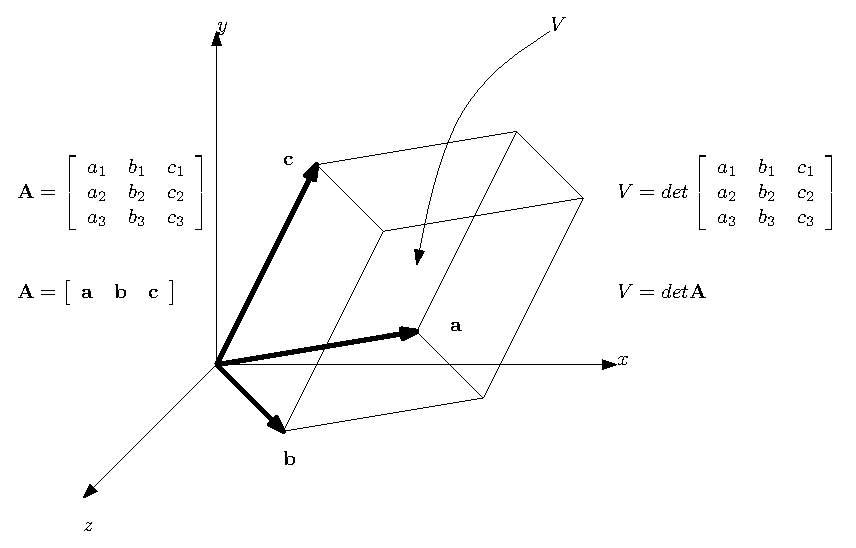
\includegraphics[width=8cm]{Math_matrix/determinantGeo3D.eps}
    \caption{3차원 공간에서 두 개의 열 벡터가 만들어내는 평행육면체의 부피}
    \label{fig:matrix:determinantGeo3D}
\end{figure}

\subsection{행렬에 대한 기하적 이해}

이제 행렬과 행렬식에 대한 기하적 개념을 정리해 보자. 이를 위해서 그림 \ref{fig:matrix:matrixConcept}를 참조하자.
그림에는 검정색 굵은 화살표로 $x$축, $y$축 $z$축이 그려져 있다.
이 축들을 벡터로 표현하면 다음과 같다.

$$
x = \left [ 
\begin{array}{c}
1 \\
0 \\
0 
\end{array}
\right ], ~~~
y = \left [ 
\begin{array}{c}
0 \\
1 \\
0 
\end{array}
\right ], ~~~
z = \left [ 
\begin{array}{c}
0 \\
0 \\
1 
\end{array}
\right ]
$$


이 세 축을 열벡터로 하는 행렬을 만들면 $3 \times 3$의 항등행렬이 된다.
이 항등행렬은 세 개의 축을 모서리로 하는 육면체 공간을 나타내고 있으며, 그 부피는 1이다.

$$\mathbf I = \left [ x~ y~ z \right ] =
\left [
\begin{array}{ccc}
1 & 0 & 0 \\
0 & 1 & 0 \\
0 & 0 & 1
\end{array}
\right ]
$$

\begin{figure}[h!]
  \centering
    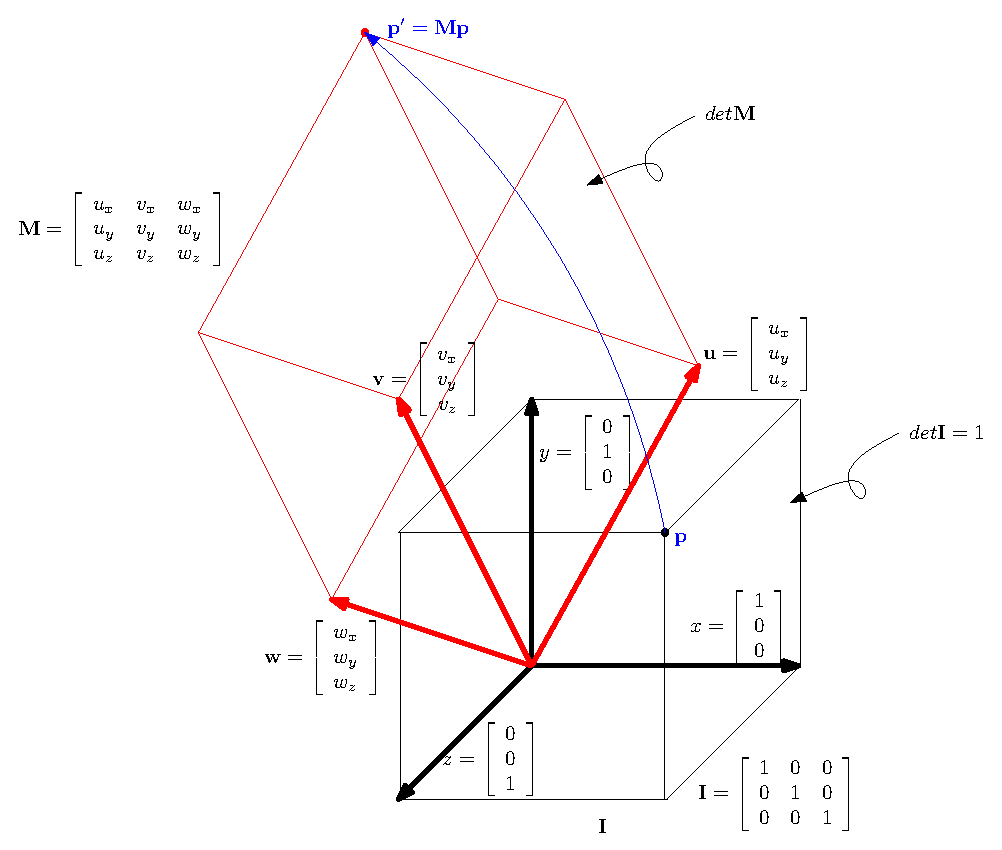
\includegraphics[width=14cm]{Math_matrix/matrixConcept.eps}
    \caption{벡터 더하기 연산의 기하적 의미}
    \label{fig:matrix:matrixConcept}
\end{figure}

이제 붉은 색으로 그려진 세 개의 축 $\mathbf u$, $\mathbf v$, $\mathbf w$를 살펴 보자.
이들을 세 개의 열 벡터로 하는 행렬 $\mathbf M$은 다음과 같다.

$$\mathbf M = \left [ \mathbf u ~ \mathbf v ~ \mathbf w \right ] =
\left [
\begin{array}{ccc}
u_x & v_x & w_x \\
u_y & v_y & w_y \\
u_z & v_z & w_z
\end{array}
\right ]
$$

이 행렬을 표현하는 세 개의 열 벡터를 모서리로 만들어지는 평행육면체가 붉은 색으로 그려져 있다.
이 육면체의 부피가 $det \mathbf M$이다.

이 행렬 $\mathbf M$은 어떤 일을 하는 것일까.
이 행렬에 세 개의 축을 곱해 보자. 다음과 같은 결과를 얻을 것이다.

$$\mathbf u = \mathbf M x, ~~~\mathbf v = \mathbf M y, ~~~\mathbf w = \mathbf M z$$

이것은 $\mathbf I$가 표현하는 부피 1의 공간(정육면체로 그려져 있는 공간)의 모든 점들에 $\mathbf M$을 곱하면
붉은 색으로 그려진 평행육면체가 표현하는 공간으로 옮겨진다는 것을 의미한다.
이 평행육면체의 부피 $det \mathbf M$은 단위 부피의 공간을 얼마나 확대하거나 축소하여 옮겨 놓는지를 알려주는 값이 된다.


어떤 좌표 $\mathbf p$가 세 축이 만들어내는 육면체의 모서리에 있다.
이 점에 $\mathbf M$을 곱하면 이것은 행렬 $\mathbf M$의 세 열 벡터가 만들어 내는 공간의 모서리 $\mathbf p'$로
옮겨가는 데, 그 값은 $\mathbf M \mathbf p$이다.


\subsection{행렬식의 특성}

몇 가지 기억해 둘 행렬식의 특성은 다음과 같다.

$$|\mathbf A| = |\mathbf A^{\rm T}|$$

$$\mathbf A \in \mathbb R^{n \times n} \Rightarrow | k \mathbf A | = k^n |\mathbf A|$$

$$|\mathbf {AB}| = |\mathbf A| |\mathbf B|$$

\section{역행렬(inverse matrix)}
\index{matrix!inverse}\index{행렬!역행렬}\index{역행렬}

역행렬은 정방행렬에만 존재한다. 어떤 행렬 $\mathbf A$가 정방행렬이고 역행렬이 존재한다면,
이 역행렬을 $\mathbf A^{-1}$로 표현한다. 이때 이 역행렬 $\mathbf A^{-1}$은 다음과 같은 조건을 만족한다.

$$\mathbf {AA}^{-1} = \mathbf I$$
$$\mathbf A^{-1} \mathbf A = \mathbf I$$

모든 정방행렬이 역행렬을 가지는 것은 아니다. 역행렬이 존재하는 행렬을 가역행렬(invertible matrix)라고 하며,
역행렬이 존재하지 않는 행렬은 특이행력(singular matrix)라고 한다.

어떤 행렬 $\mathbf A$가 정방행렬이 아니고 $\mathbb R^{m \times n}$에 속한다고 하자.
다른 어떤 행렬 $\mathbf B$가 $\mathbb R^{n \times m}$에 속하면, 두 행렬의 곱 $\mathbf {AB}$는 $\mathbb R^{m \times m}$에 속하는 정방행렬이
된다. 만약 $\mathbf {AB} = \mathbf I \in \mathbb R^{n \times n}$이라면,
$\mathbf B$를 $\mathbf A$의 의사 역행렬(pseudo-inverse)라고 한다.

\subsection{역행렬의 계산}

역행렬의 계산은 수반행렬(adjoint matrix)를 이용하여 쉽게 정의할 수 있다.
어떤 행렬 $\mathbf A$의 수반행렬을 $adj \mathbf A$로 표현하며, 이 수반행렬은 여인자를 이용하여 다음과 같이 정의된다.

\begin{itemize}
\item 행렬 $\mathbf A$의 수반행렬: 행렬 $\mathbf A$의 $i$ 행과 $j$ 열에 대해 정의되는 여인자 $C_ij$를 $j$ 행 $i$ 열 성분으로 하는 행렬.
\end{itemize}

따라서 수반행렬은 $C_{ij}$를 성분으로 $i$행 $j$열 성분으로 하는 행렬 $\mathbf C$의 전치(transpose)이며, 다음과 같다. 

\begin{eqnarray}
adj \mathbf A = 
\left (
\begin{array}{cccc}
C_{11} & C_{21} & \cdots & C_{n1} \\
C_{21} & C_{22} & \cdots & C_{n2} \\
\vdots & \vdots & \ddots & \vdots \\
C_{n1} & C_{2n} & \cdots & C_{nn} \\
\end{array}
\right )
= \mathbf C^{\rm T}
\end{eqnarray}
 
수반행렬이 구해지면 다음과 같이 이 수반행렬을 행렬의 행렬식으로 나누면 역행렬이 된다.

\begin{eqnarray}
\mathbf A^{-1} = \frac{adj \mathbf A}{|\mathbf A|} = 
\frac{1}{|\mathbf A|}
\left (
\begin{array}{cccc}
C_{11} & C_{21} & \cdots & C_{n1} \\
C_{21} & C_{22} & \cdots & C_{n2} \\
\vdots & \vdots & \ddots & \vdots \\
C_{n1} & C_{2n} & \cdots & C_{nn} \\
\end{array}
\right )
= \mathbf C^{\rm T}
\end{eqnarray}

식은 간단하지만, 여인자를 구하려면 재귀적으로(recursively) 계속하여 작은 행렬의 여인자를 구해나가야 하므로 실제 계산에 필요한 자원이 매우 큰 문제가 된다.
